\DiaryEntry{Queuing Theory, Applications}{2019-09-05}{Stochastic}

Before we continue with the infinite queue with one server, we cover some relations which are valid for any queue.

\subsection{Little's Law}

Little's law relates the expected number of jobs in the system, $E(N)$, with the mean time jobs spend in the system, $E(T)$ as follows,

\bee
E(N) = \lambda E(T)
\eee

where $\lambda$ is the average arrival rate of the system. This law is \emph{independent} from the arrival process, service time distribution, network topology, and service order!

Intuitively, the law makes sense: In a fast-food restaurant, $E(T)$ will be low (people get and eat their food quickly), therefore not many people are in the fast-food restaurant; i.e. $E(N)$ is low as well. In a slow-service restaurant, $E(T)$ will be hig (people wait longer for their food) and therefore, more people will be in the restaurant and $E(N)$ will therefore be higher.


\subsection{Infinite Queue with one Server}

Recall the expression for the limiting distribution $\pi_i$ from the previous entry,

\bee
\pi_i = \left( 1 - \frac{\lambda}{\mu} \right) \left(\frac{\lambda}{\mu}\right)^i = \rho^i (1-\rho)
\eee

where we have introduced the utilization $\rho$ as $\rho = \frac{\lambda}{\mu}$. We can use this expression to calculate the mean number of jobs in the system, $E(N)$,

\bee
E(N) = \sum_{i=0}^\infty i \pi_i = \sum_{i=1}^\infty i \rho^i(1-\rho) = (1-\rho) \sum_{i=1}^\infty i \rho^i = \rho (1-\rho) \sum_{i=1}^\infty i \rho^{i-1}
\eee

We can use now the standard trick to recognize the sum expression as $d \rho^i / di$ and can rewrite the expression as

\bee
E(N) = \rho (1-\rho) \sum_{i=1}^\infty \frac{\rho^{i}}{di} = \rho(1-\rho) \frac{d}{di} \sum_{i=1}^\infty \rho^{i} = \rho(1-\rho) \frac{d}{di} \left( \frac{1}{1-\rho} \right) = \rho (1-\rho) \frac{1}{(1-\rho)^2} = \frac{\rho}{1-\rho} \qed
\eee

The variance can be shown to be

\bee
\text{Var}(N) = \frac{\rho}{(1-\rho)^2}
\eee

From the mean expression, we can calculate the mean time in the system (by means of Little's law),

\bee
E(T) = \frac{E(N)}{\lambda} = \frac{1}{\mu - \lambda}
\eee

and the mean time a job waits in the queue as

\bee
E(T_Q) = E(T) - \frac{1}{\mu} = \frac{\rho}{\mu - \lambda}
\eee

All these expressions increase sharply, when the arrival rate comes near the mean job processing duration; $\lambda \rightarrow \mu$; i.e. the system becomes overloaded.

\paragraph{Simulation Results.} The Julia file \href{https://github.com/ClemensFMN/JuliaStuff/blob/master/SimJulia/simple_queue.jl}{here} contains a simulation using the SimJulia framework.

The first Figure shows the histogram of $T$ for $\lambda=2, \mu=5 $ which follows an exponential distribution. The expected value $E(T)=\frac{1}{\mu - \lambda} = \frac{1}{3}$ matches the simulation value ($0.33$) quite closely.

\begin{figure}[hbt!]
\centering
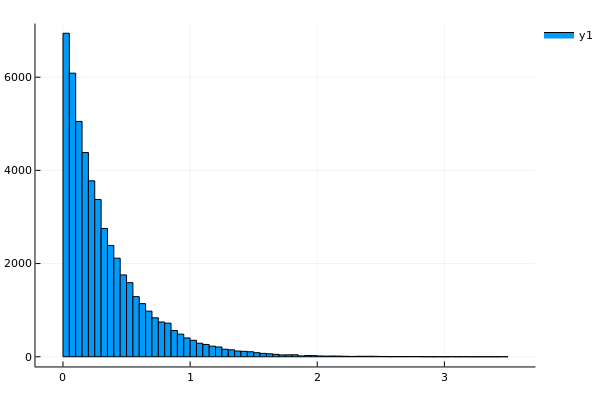
\includegraphics[scale=0.4]{images/queuing_3_1.png}
\end{figure}

Simulation allows experimenting with other distributions for the arrival and / or job processing process.

As a simple first example, we consider a system with exponential interarrival times ($\lambda = 0.1$) and deterministic processing time $=1.0$. The following Figure shows the processing time per job for this case on the left. Since the arrivals are very seldom compared to the processing time, most jobs are processed without queuing (therefore the total time in the system is $1.0$). Only a small number of jobs need to queue and their processing time is therefore longer. If we increase the arrivals to $\lambda=0.8$, most of the jobs need to queue and the processing time increases as shown in the following Figure on the right.


\begin{figure}[hbt!]
\centering
\begin{subfigure}{.5\textwidth}
  \centering
  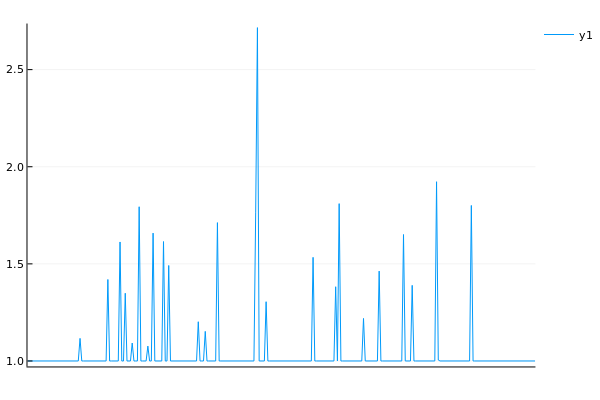
\includegraphics[width=.9\linewidth]{images/queuing_3_3.png}
  \caption{Processing time per job, $\lambda=0.1$}
  \label{fig:sub1}
\end{subfigure}%
\begin{subfigure}{.5\textwidth}
  \centering
  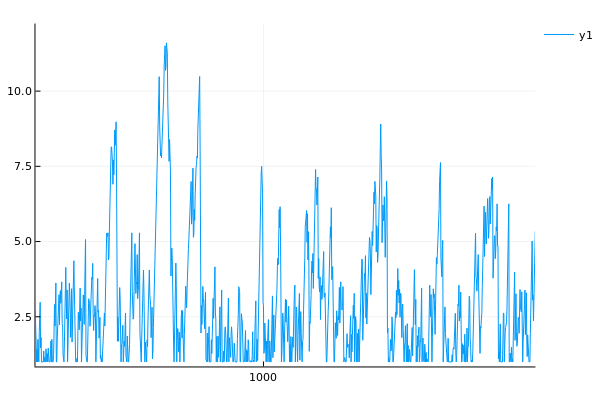
\includegraphics[width=.9\linewidth]{images/queuing_3_4.png}
  \caption{Processing time per job, $\lambda=0.8$}
  \label{fig:sub2}
\end{subfigure}
\end{figure}


Finally, we consider a system with exponential interarrival times, $\lambda = 2$ and uniform job processing distribution (uniform in the interval $[0,0.4]$ so that the mean is the same as of the exponential job processing distribution from before). The following Figure shows the histogram of $T$.

\begin{figure}[hbt!]
\centering
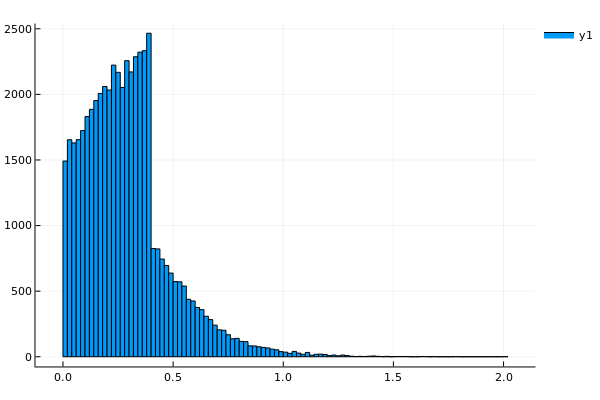
\includegraphics[scale=0.4]{images/queuing_3_2.png}
\end{figure}

Since the uniform distribution has finite support there are no jobs running longer than $0.4$ and we therefore expect the mean of $T$ to be shorter (simulation yields $0.288$); however, the histogram looks quite different.

%%% Local Variables:
%%% mode: latex
%%% TeX-master: "journal"
%%% End:
